\documentclass[letterpaper,11pt]{article}
\oddsidemargin -1.0cm \textwidth 17.5cm

\usepackage[utf8]{inputenc}
\usepackage[activeacute,spanish, es-lcroman]{babel}
\decimalpoint
\usepackage{amsfonts,setspace}
\usepackage{amsmath}
\usepackage{amssymb, amsmath, amsthm}
\usepackage{comment}
\usepackage{float}
\usepackage{amssymb}
\usepackage{dsfont}
\usepackage{anysize}
\usepackage{multicol}
\usepackage{enumerate}
\usepackage{graphicx}
\usepackage[left=1.5cm,top=2cm,right=1.5cm, bottom=1.7cm]{geometry}
\setlength\headheight{1.5em} 
\usepackage{fancyhdr}
\usepackage{multicol}
\usepackage{hyperref}
\usepackage{wrapfig}
\usepackage{subcaption}
\usepackage{siunitx}
\usepackage{cancel}
\usepackage{mdwlist}
\usepackage{svg}
\pagestyle{fancy}
\fancyhf{}
\renewcommand{\labelenumi}{\normalsize\bfseries P\arabic{enumi}.}
\renewcommand{\labelenumii}{\normalsize\bfseries (\alph{enumii})}
\renewcommand{\labelenumiii}{\normalsize\bfseries \roman{enumiii})}


\begin{document}

\fancyhead[L]{\itshape{Facultad de Ciencias F\'isicas y Matem\'aticas}}
\fancyhead[R]{\itshape{Universidad de Chile}}
\rfoot[]{pág. \thepage}

\begin{minipage}{11.5cm}
    \begin{flushleft}
        \hspace*{-0.6cm}\textbf{FI1000-1 Introducción a la Física Clásica}\\
        \hspace*{-0.6cm}\textbf{Profesor:} Ignacio Bordeu\\
        \hspace*{-0.6cm}\textbf{Auxiliares:} Alejandro Cartes \& Simón Yáñez\\
        \hspace*{-0.6cm}\textbf{Ayudante:} Javier Cubillos\\
    \end{flushleft}
\end{minipage}

\begin{picture}(2,3)
    \put(366, 10){
\includegraphics[scale=0.9]{2020-1/Imágenes/logo/dfi-fcfm.pdf}}
\end{picture}

\begin{center}
	\LARGE\textbf{Auxiliar \#8}\\
	\Large{De todito}
\end{center}

\vspace{-1cm}
\begin{enumerate}\setlength{\itemsep}{0.4cm}

\item[]

\item Un bloque de masa $m_a$ está situado sobre un plano horizontal. El coeficiente de fricción cinética entre el bloque y el plano es $\mu_c$. El bloque está unido a una cuerda que pasa a través de dos poleas y acaba atada al techo. Una de las poleas lleva unido un bloque de masa $m_b$ como indica la figura. Teniendo en cuenta que la masa de las poleas y la cuerda es despreciable, determinar la aceleración de los bloques $A$ y $B$ y la tensión de la cuerda.

    \begin{figure}[H]
        \centering
        \svgpath{../../2023-1/img/aux_8/}
        \includesvg[width=\linewidth]{Aux 8 - P1.svg}
    \end{figure}

\newpage
\item Determinar el valor de la velocidad angular máxima y mínima de giro del cono de la figura para que un objeto de masa $m$ no se deslice por su pared. El coeficiente de fricción estático es $\mu_e$ y el radio de la circunferencia que describe es $R$.

        

    \begin{figure}[H]
        \centering
        \svgpath{../../2023-1/img/aux_8/}
        \includesvg[width=\textwidth]{Aux 8 - P2.svg}
    \end{figure}
    
    

\item \textbf{[C2 - Otoño 2022]} Un resorte de constante elástica $k$, de largo natural $l_0$, tiene uno
de sus extremos unido a una bola de masa $m$. Su otro extremo $A$ está sujeto a un
brazo horizontal de longitud $d$ que rota de tal forma que la bola se encuentra en un
movimiento circular uniforme de radio constante cuando el largo del resorte es $L$.

\begin{enumerate}
    \item Determine el ángulo $\theta$ que forma el resorte con la vertical
    \item Determine la rapidez $v$ de la bola
\end{enumerate}


\begin{figure}[H]
    \centering
    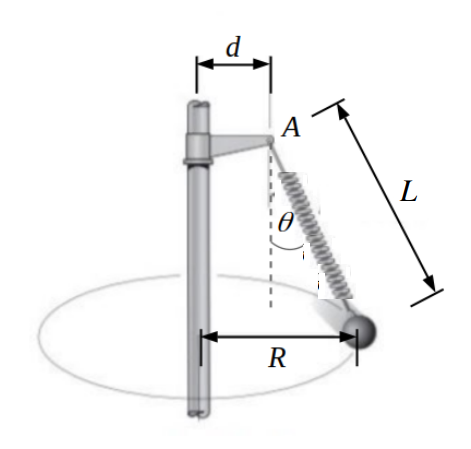
\includegraphics[width = 0.4\textwidth]{2023-1/img/aux_8/Aux 8 - P3.PNG}
\end{figure}

% Para imágenes vectoriales -> el texto tiene que estar en LaTeX
% \begin{figure}[htbp]
%   \centering
%   \svgpath{../Imagenes/ejercicios}  -> .. irse pa'trás 
%   \includesvg{ej5.svg}
% \end{figure}
\end{enumerate}
\end{document}